\subsection{Abuse Detection}
This is a single-class classification problems. The challenge is to detect when a comment from a conversation would be considered insulting to another participant in the conversation. The idea is to create a generalisable single-class classifier which could operate in a near real-time mode. Classification is a form of supervised learning, it takes a set of data ${X, Y}$ where $X$ is a set of attributes and $Y$ is the target class. The goal is to model $Y$ as a function of $X$, $y = f(x)$, where $x \in X$ is a specific sample and $y \in Y$ is the corresponding class for that sample.

Abuse detection is primarily implemented in python, consisting of multiple scripts. The script requires python version 2.7 or above to executes due to certain dependencies and functions used. The script makes use of multiple Python libraries including Sci-kit learn \cite{scikit:home}, NLTK \cite{nltk}, Numpy \cite{Numpy} and Pandas \cite{Pandas}, and others such as mysql, which provide machine learning models and objects for loading and processing the data. The code for this functionality has been modularised and is thus split across various files and classes. This allows modules to be included, instantiated, upgraded and reused whenever necessary.

\subsubsection{Data Description}
As mentioned previously, classification is a form of supervised learning. This means that a dataset is required to train the classifier which can then be used to make predictions on unseen instances, based on the training data. A suitable dataset was found online, provided by Impermium and hosted on the popular machine learning competitions site Kaggle \cite{Kaggle:Dataset}. The dataset was split into two files, train.csv and test.csv, and consisted of three attributes: Insult, Date, Comment. The training set contains 3,948 samples and would be used to train the models whereas the test set contains 2,648 samples and would be used to verify the accuracy of the model.


\subsubsection{Data Preprocessing}
As the data has been downloaded from a third-party, we must ensure that it is in the correct format. The data preprocessing stage will ensure that all the training and test data is consistent with the data we expect on the social network. This step is only carried during the training phase.

 The dataset was loaded into memory as a table (DataFrame) using the Pandas library. The library provided a function to read CSV files with headers as demonstrated in figure \ref{fig:AbuseDetection_LoadData}. A generic function was created for loading in the dataset as this functionality is required multiple times, for loading the test and training datasets separately.

\begin{figure}[H]
	\centering
	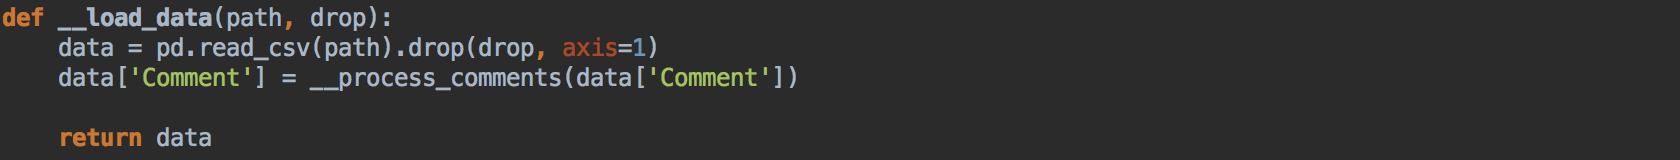
\includegraphics[width=\textwidth]{Images/Implementation/DataProcessing/AbuseDetection/LoadData}
	\caption{Function that cleans a post}
	\label{fig:AbuseDetection_LoadData}
\end{figure}

The raw dataset contains multiple errors which will effect the accuracy of the resulting model. As a result, before the data can be used, it needs to be processed and cleaned. For example, there are comments which contain several ascii characters that have been encoded. Similarly, there are several comments which contain underscores and new line characters that must be stripped so the ngrams can be generated correctly.

\begin{figure}[H]
	\centering
	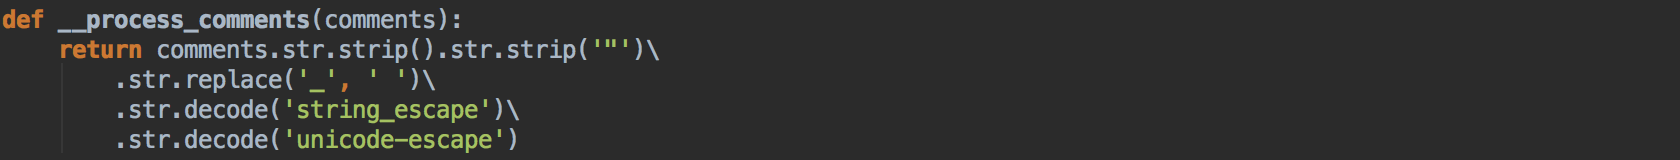
\includegraphics[width=\textwidth]{Images/Implementation/DataProcessing/AbuseDetection/ProcessComments}
	\caption{Function that cleans a post}
	\label{fig:AbuseDetection-ProcessComments}
\end{figure}

The function in figure \ref{fig:AbuseDetection-ProcessComments} processes the entire DataFrame in one go, firstly stripping any white space on the edges, then replacing all the underscores with spaces. The resulting string is then first decoded using string\_escape, which produce a string that is suitable as string literal in Python source code and then decoded using unicode\_escape, which produce a string that is suitable as Unicode literal in Python source code \cite{Python:Codes}.

\begin{figure}[H]
	\centering
	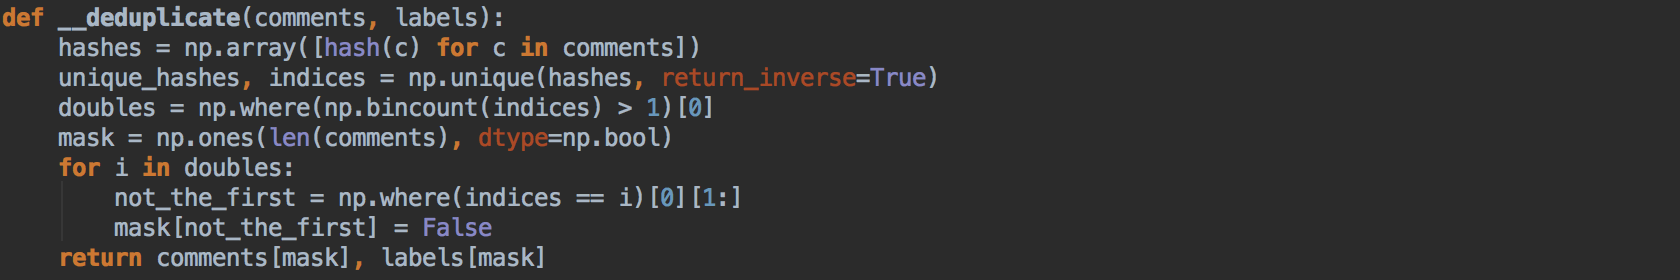
\includegraphics[width=\textwidth]{Images/Implementation/DataProcessing/AbuseDetection/Deduplicate}
	\caption{Function that cleans a post}
	\label{fig:AbuseDetection-Deduplicate}
\end{figure}

The next step involved cleansing the data by removing any duplicate comments in the training set. The function in figure \ref{fig:AbuseDetection-Deduplicate} takes a set of comments and their labels to filter out duplicated comments, returning only unique comments with their associated labels. The first part of this process computes the hash of every comment. This will result in the same hash for two comments that are identical, due to the nature of the hashing process. Next, we take the indices of all the unique hashes, which returns bins containing the indices corresponding to every hash value. As a result, if a hash appears twice then it will contains two indices in its bin. The indices of the hashes are then used to find the duplicates where the bin has more than indices in it. Given all the duplicates, we can generate a mask, lines 5-8, which only returns one instance of every duplicate comment. Finally, the mask is used to access all the unique comments and their associated labels.

\subsubsection{Feature Engineering}
The raw data, a sequence of symbols cannot be fed directly to the algorithms themselves as most of them expect numerical feature vectors with a fixed size rather than the raw text documents with variable length \cite{scikit:tfidf}. In order to achieve a reasonable accuracy, the features of the dataset must be transformed into something meaningful.


\begin{figure}[H]
	\centering
	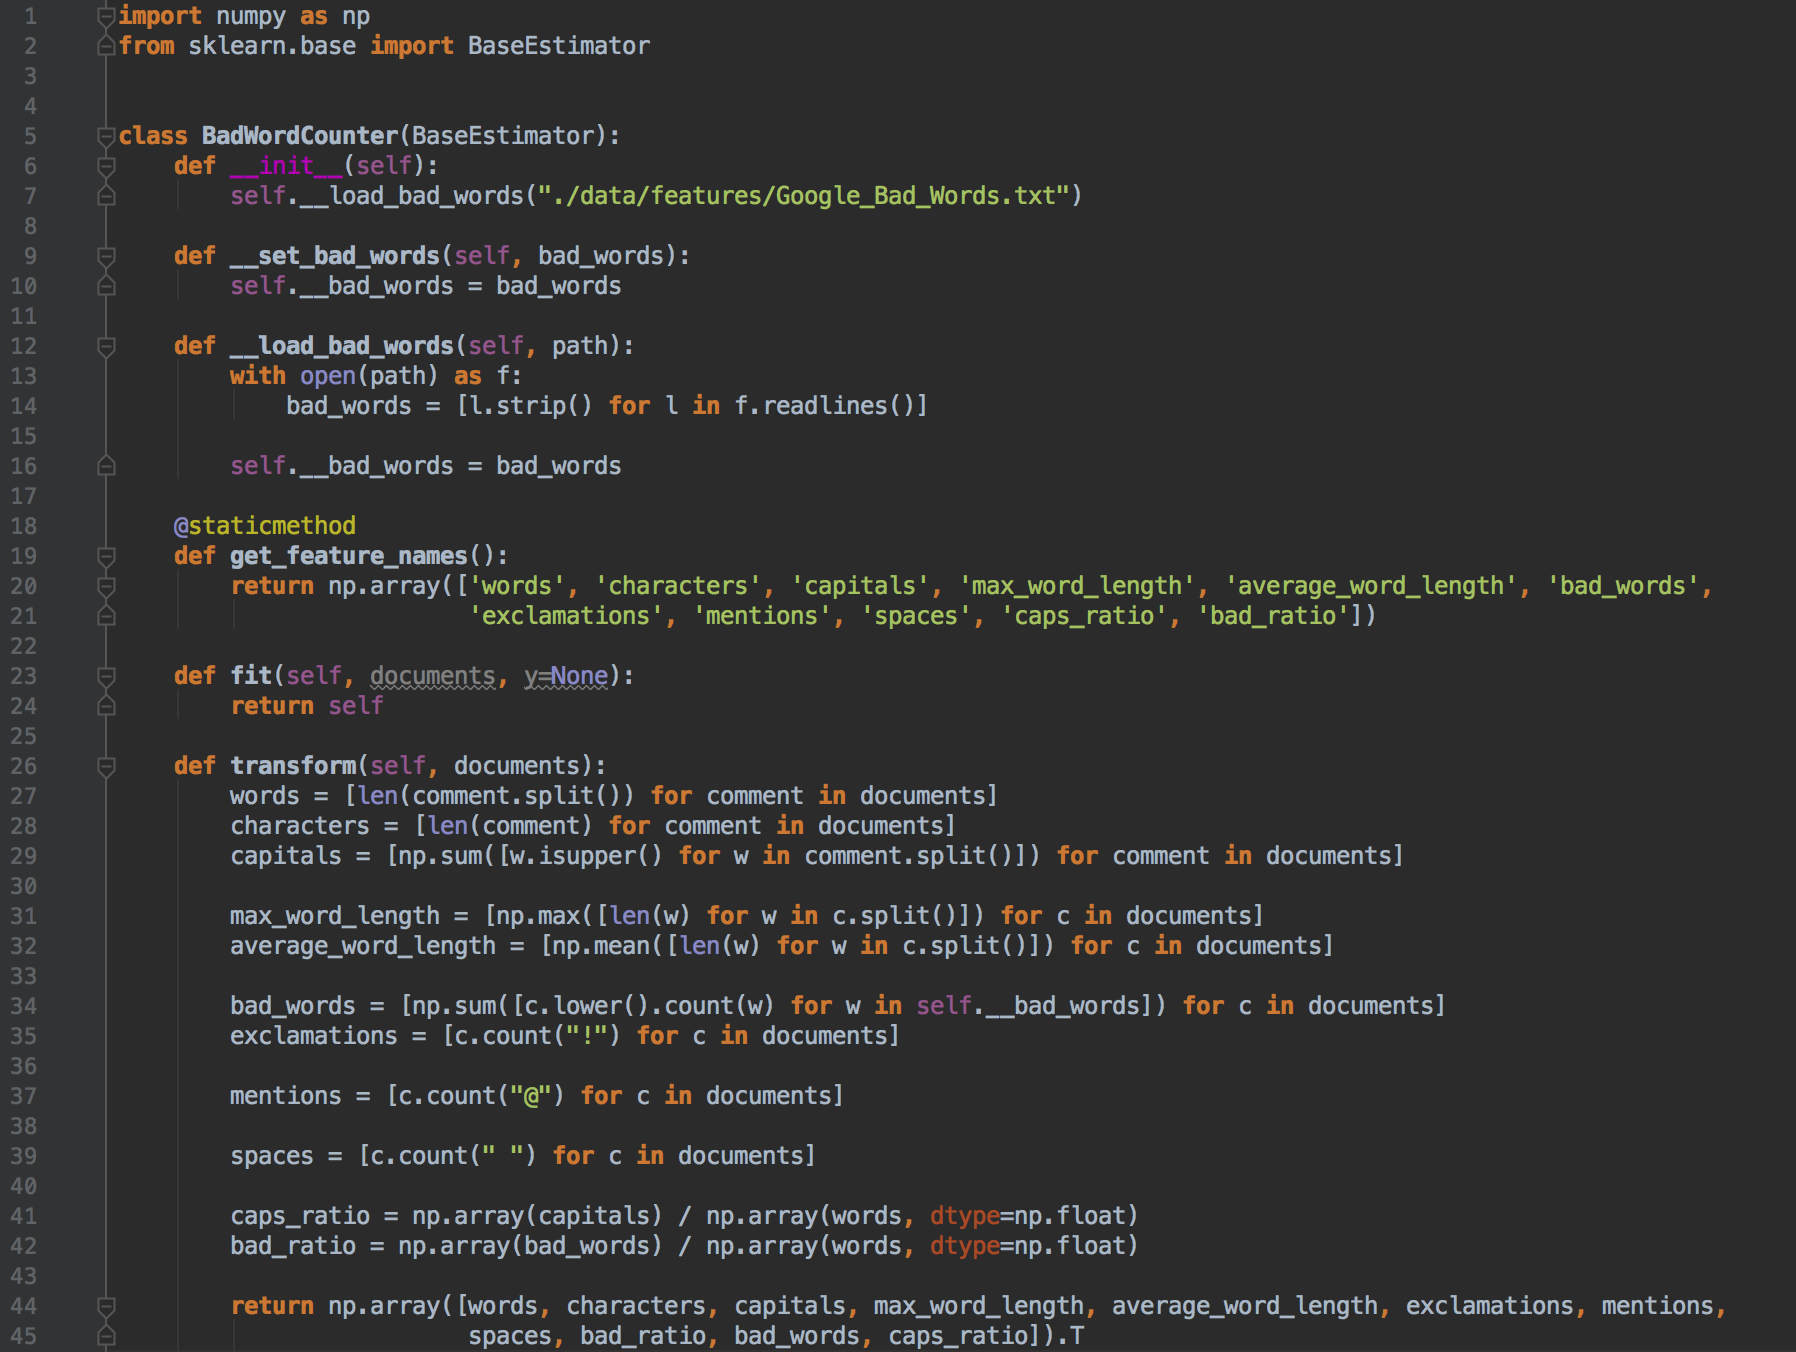
\includegraphics[width=\textwidth]{Images/Implementation/DataProcessing/AbuseDetection/BadWordCounter}
	\caption{Function that cleans a post}
	\label{fig:AbuseDetection-BadWordCounter}
\end{figure}

\paragraph{Bad Word Counter} This feature engineering technique takes advantage of a list of the commonly used ``inappropriate'' words. The list was originally developed by Google for their ``What do you love'' project \cite{GitHub:GoogleBadWordList}. It contains 451 words which Google considered inappropriate and banned from being displayed on the project. The transformer was implemented using a new class which implements the BaseEstimator interface, more specifically, the fit and transform methods of the BaseEstimator. As applying this transformation results in a completely new set of features which are independent for every sample, the fit method is not necessary and is therefore not actually implemented. There are currently eleven unique features generated, some more important than others but this is up to the classifier to decide. All the features returned are numerical (either integer or float).

The class starts by loading the Bad Words List (BWL), in the constructor, when the class is instantiated. The transform function accepts a list of documents (comments) and returns a two dimensional array with $|documents| \times |features|$ elements. Lines 27, 28, 29 compute the number of words, characters and uppercase words in each comment. Lines 31 and 32 then proceed to compute the length of the longest word and the average word length for each comment. These features are pretty generic and don't necessarily indicate any abusive comments but the model may find a pattern so we can include them for safety. The next features generated are the number of bad words based on the BWL and the number of exclamation marks in each comment. These two features are quite indicative of an abusive comment. Next we compute a few more generic features including the number of mentions (users) and the number of spaces. Lastly, we compute the caps to non-caps ratio and the bad to normal words ratio and represent them as floats to indicate the severity of post. Finally, we combine all these features and return a 2D matrix.

\paragraph{TFIDF Vectoriser} This is the process of converting a collection of raw documents to a matrix of TF-IDF features. It is equivalent to using a CountVectorizer followed by TfidfTransformer \cite{ScikitLearn:TFIDFVectorizer}. 

The CountVectorizer in the scikit-learn package generates features by tokenising strings giving an integer id for each possible token, counting the occurrences of tokens in each document, and then normalising and weighting with diminishing importance tokens that occur in the majority of samples/documents \cite{scikit:tfidf}. We call vectorisation the general process of turning a collection of text documents into numerical feature vectors. This specific strategy (tokenisation, counting and normalisation) is called the Bag of Words or ``Bag of n-grams'' representation. Documents are described by word occurrences while completely ignoring the relative position information of the words in the document \cite{scikit:tfidf}.

In large comments, some words will appear very often (e.g. ``the'', ``a'', ``an'', etc). These words have very little meaning in terms of the classification process. Feeding these terms directly into the classifier would result in these very frequent meaningless overshadowing the less frequent meaningful terms. Tf means term-frequency while TF-IDF means term-frequency times inverse document-frequency \cite{scikit:tfidf}. The TFIDF transformer simply re-weights the count features into floating point values, suitable for usage by a classifier, by multiplying the term frequency with the IDF component. The IDF component can be computed using the equation \ref{equation:IDF}, where $n_{d}$ is the total number of documents, and $df(d,t)$ is the number of documents that contain term $t$. The resulting TF-IDF vectors are then normalised by the Euclidean norm.

\begin{equation}
	idf(t) = log\frac{1 + n_{d}}{1 + df(d, t)} + 1
	\label{equation:IDF}
\end{equation}

Two separate set of TF-IDF features were generated, one for words and one for for characters. The \textit{analyser} can be tweaked which determines whether the feature should be made of word or character n-grams. The \textit{ngram\_range} parameter takes a lower and upper boundary of the range of n-values for different n-grams to be extracted. All values of n such that $min\_n <= n <= max\_n$ will be used. The \textit{binary} value of $False$ ensures that frequencies of zero are not normalised to one.

\begin{figure}[H]
	\centering
	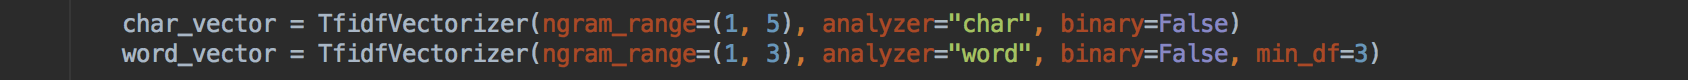
\includegraphics[width=\textwidth]{Images/Implementation/DataProcessing/AbuseDetection/TFIDF}
	\caption{Function that cleans a post}
	\label{fig:AbuseDetection-TFIDF}
\end{figure}

\subparagraph{Characters} The character vectoriser uses the character analyser to generate ngrams for different combinations of characters in the comment. This vectoriser uses an \textit{ngram\_range} of 1-5, extracting character sequences at least one character long.

\subparagraph{Words} The word vectoriser uses the word \textit{analyser} which produces tokens on delimiters, such as white spaces and punctuation. Additionally, it uses an \textit{ngram\_range} of 1-3. The main difference here is that it uses the \textit{min\_df} value of 3, producing a vocabulary ignoring terms that have a document frequency strictly lower than the given threshold.

\paragraph{Feature Stacking}
asas

\begin{figure}[H]
	\centering
	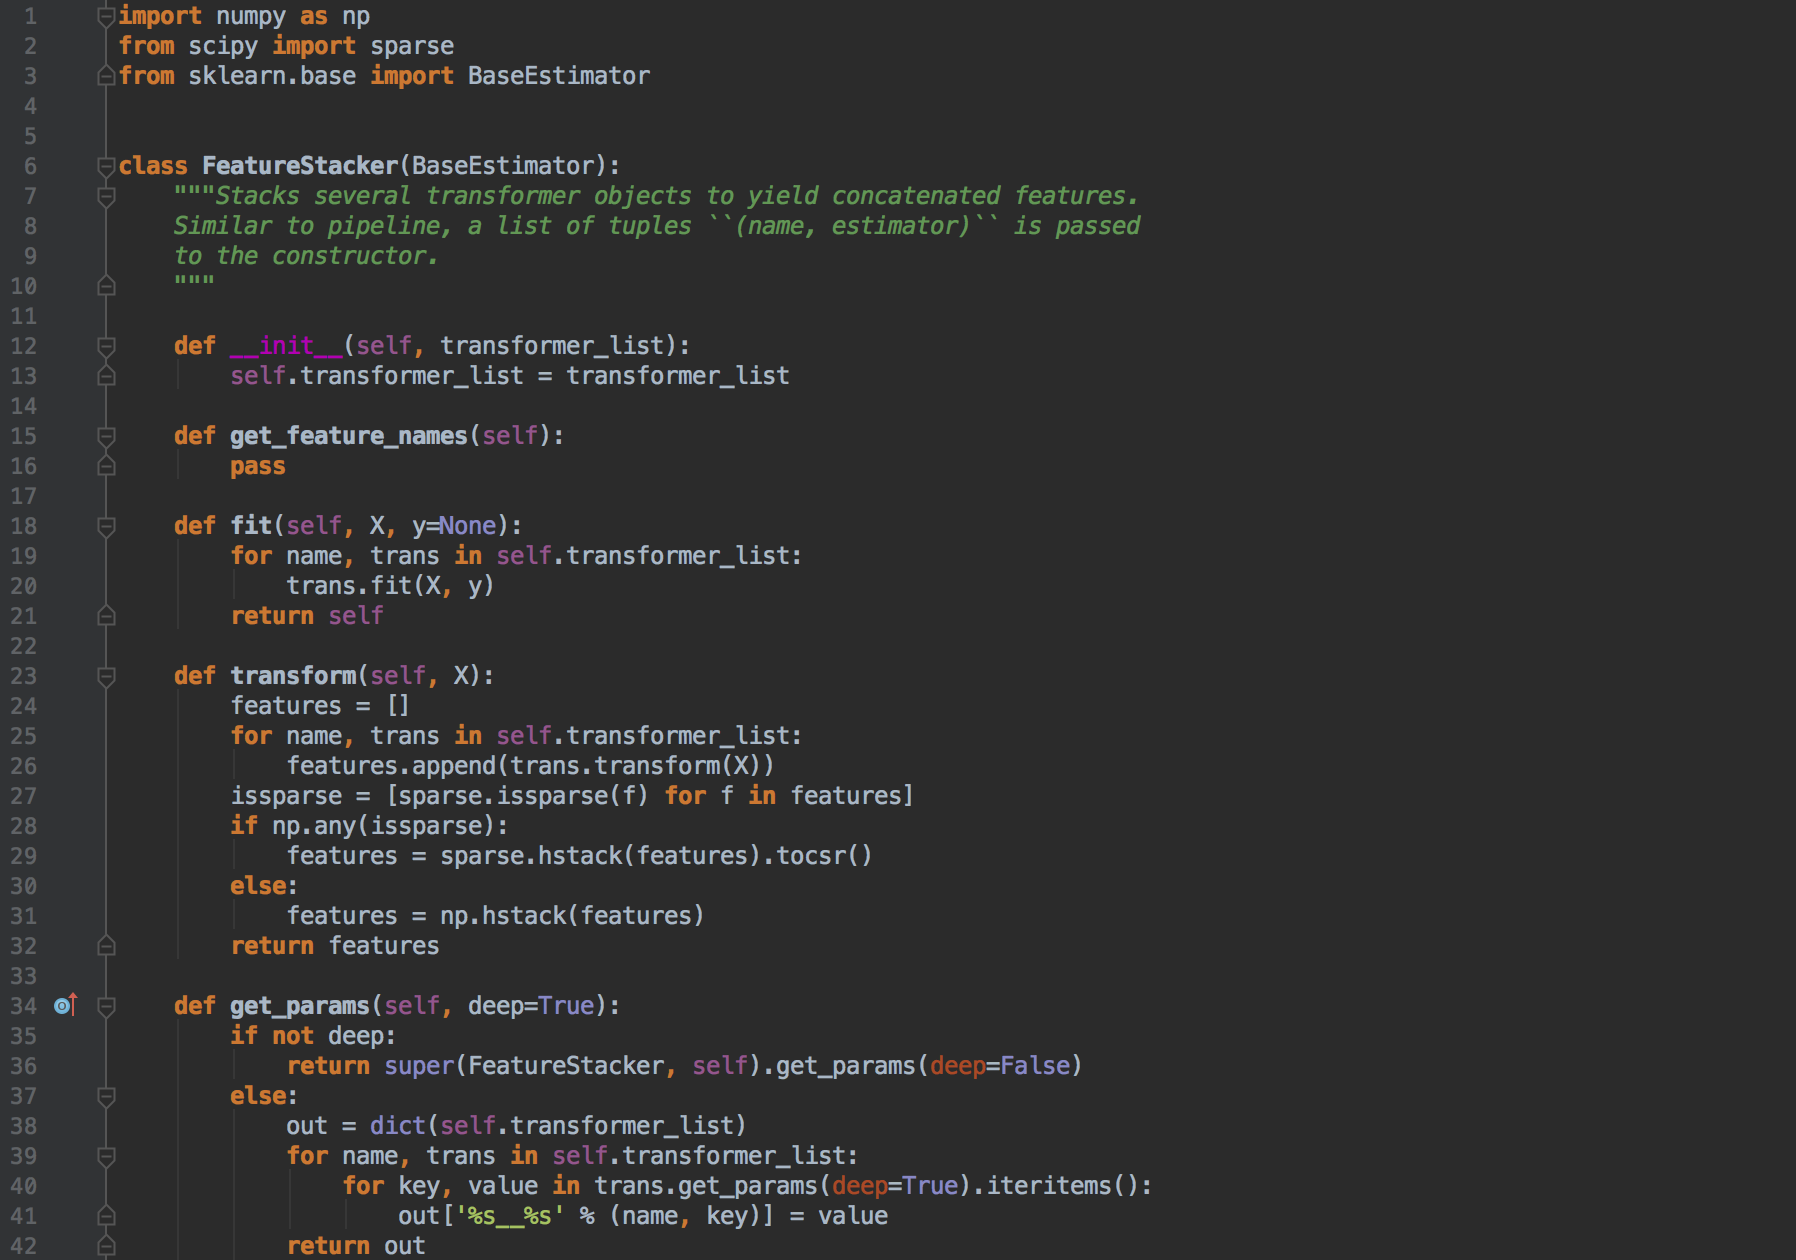
\includegraphics[width=\textwidth]{Images/Implementation/DataProcessing/AbuseDetection/FeatureStacker}
	\caption{Function that cleans a post}
	\label{fig:AbuseDetection-FeatureStacker}
\end{figure}

\subsection{Feature Selection}


\subsubsection{Modelling}

\subsubsection{Training}

\subsubsection{Predicting}

SVC Accuracy: 0.767661708092

